
% !TEX root = ../main_lecture_notes.tex
\chapter{Chaine de Markov en temps continu}\label{chap:processus_markov}
On s'intéresse dans ce chapitre à l'extension des chaine de Markov en temps continu. Le contenu de ce chapitre s'inspire des notes de cours de \citet{Truquet_stat_proc} et de l'ouvrage de \citet{Dobrow2016}.
\section{Definition}
Soit $(\Omega, \F,\F_t,\Prob)$ un espace de probabilité filtré et $X$ un processus stochastique $\F_t-$adapté à valeur sur un espace d'état dénombrable $E$.
\begin{definition}
Le processus $X$ est un processus de Markov si 
$$
\Prob(X_{t+s} = y|X_s = x, \mathcal{F}_s) = \Prob(X_{t+s} = y|X_s = x),\text{ }\forall s,t\geq 0,\text{ et }x,y \in E.
$$
Le processus de Markov $X$ est dit homogène si de plus
$$
\Prob(X_{t+s} = y|X_s = x) = \Prob(X_{t} = y|X_0 = x).
$$
\end{definition} 
Les probabilités de transition peuvent donc être placées dans des matrices de transition indicées sur le temps $(P_t)_{t\geq 0}$, définies par 
$$
P_t = (p_t(x,y))_{x,y\in E} = (\Prob(X_t = y|X_0 = x))_{x,y\in E}
$$
Soit $X$ un processus de Markov de probabilité de transition $(p_t)_{t\geq0}$. On retrouve les mêmes propriétés que pour les chaines de Markov, par exemple les équations de Chapman-Kolmogorov.
\begin{prop}\label{prop:CK}
$$
P_{t+s} = P_{t}P_s\text{, }\forall s,t\geq0.
$$
\end{prop}
\begin{proof}
Soit $(x,y)\in E^2$
\begin{eqnarray*}
p_{t+s}(x,y) &=& \Prob(X_{s+t} = y|X_0 = x)\\
&=&\sum_{z\in E}\Prob(X_{s+t} = y,X_{s} = z|X_0 = x)\\
&=&\sum_{z\in E}\Prob(X_{s+t} = y|X_{s} = z,X_0 = x)\Prob(X_{s} = z|X_0 = x)\\
&=&\sum_{z\in E}\Prob(X_{s+t} = y|X_{s} = z)\Prob(X_{s} = z|X_0 = x)\\
&=&\sum_{z\in E}\Prob(X_{t} = y|X_{0} = z)\Prob(X_{s} = z|X_0 = x)\\
&=&\sum_{z\in E}p_s(x,z)p_t(z,y)\\
\end{eqnarray*}
\end{proof}
\begin{ex}
Le processus de Poisson $N$ d'intensité $\lambda$ est un processus de Markov sur $\N$! La propriétés d'accroissements indépendants et stationaires implique la propriété de Markov. On a, pour $(i,j)\in \N^2$ tels que  $i\leq j$ et $s,t\geq 0$,
\begin{eqnarray*}
\Prob(N_{s+t} = j|N_s =i)&=&\frac{\Prob(N_{s+t} = j,N_s =i)}{\Prob(N_s =i)}\\
&=&\frac{\Prob(N_{s+t} - N_s = j-i, N_s =i)}{\Prob(N_s =i)}\\
&=&\frac{\Prob(N_{s+t} - N_s = j-i)\Prob(N_s =i)}{\Prob(N_s =i)}\\
&=&\Prob(N_{s+t} - N_s = j-i)\\
&=&\Prob(N_{t} = j-i) = p_t(i,j) = \frac{e^{-\lambda t}(\lambda t)^{i-j}}{(j-i)!}.\\
\end{eqnarray*} 
Les matrices des transitions est de dimension infini 
$$
P_t = \left(
\begin{array}{cccc}
\e^{-\lambda t}&(\lambda t)\e^{-\lambda t}&(\lambda t)^2\e^{-\lambda t}/2&\cdots\\
0&\e^{-\lambda t}&(\lambda t)\e^{-\lambda t}&\cdots\\
0&0&\e^{-\lambda t}(\lambda t)&\cdots\\
\vdots&\vdots&\vdots&\ddots
\end{array}
\right).
$$
\end{ex}
\section{Propriétés}\label{ssec:property_markov_process}
Soit $X$ un processus de Markov homogène sur $E$ tel que $X_0=x\in E$ et soit $T_x=\inf\{t\geq 0\text{ ; }X_t\neq x\}$ le temps de séjour du processus dans l'état $x\in E$.
\begin{prop}
$T_x$ est de loi exponentielle.
\end{prop}
\begin{proof}
L'idée est de montrer que la loi de $T_x$ du processus $X$ est sans mémoire. On a 
\begin{eqnarray*}
\Prob(T_x>s+t|T_x>s, X_0  =x)&=&\Prob(T_x>s+t| X_u =x,0\leq u\leq s)\\
&=&\Prob(X_u =x,0\leq u\leq s+t| X_u =x,0\leq u\leq s)\\
&=&\Prob(X_u =x,s\leq u\leq s+t| X_u =x,0\leq u\leq s)\\
&=&\Prob(X_u =x,s\leq u\leq s+t| X_s =x)\text{ (Propriété de Markov)}\\
&=&\Prob(X_u =x,0\leq u\leq t| X_0 =x)\text{ (Homogénéité dans le temps)}\\
&=&\Prob(T_x>t| X_0 =x). \\
\end{eqnarray*}
La seule distribution sur $\RL_+$ vérifiant cette propriété est la loi exponentielle.
\end{proof}
Supposons que $T_x\sim\ExpDist(q_x)$, 
\begin{itemize}
	\item Si $q_x = 0$ alors le processus reste pour toujours dans l'état $x$ qui est dit absorbant
	\item Si $q_x = \infty$ alors le processus quitte l'état $x$ tout de suite après l'avoir atteint. Le processus peut alors effectuer un nombre de transition infini sur un intervalle de temps fini. Un tel processus est dit explosif.
\end{itemize}
Supposons que $q_x\in(0,\infty)$. La question est alors de savoir quel est l'état visité après l'état $x$. L'interprétation est la suivante: 
\begin{itemize}
	\item Le processus démarre dans l'état $x\in E$
	\item Soit $T_{x,y}\sim\ExpDist[q(x,y)]$ pour $y\in E$ tel que $y\neq x$. Les paramètres $q(x,y)$ sont les taux de transitions. Si il est impossible d'aller de $x$ à $y$ directement alors $q(x,y) = 0$ et $T_{x,y} = \infty$.
	\item L'état visité après $x$ est $y^\ast = \underset{y\neq x}{\argmin} T_{x,y}$.
	\item La première alarme exponentielle qui sonne indique l'état d'arrivée du processus.
	\item On note que $T_x = \underset{y\neq x}{\min} T_{x,y}\sim\ExpDist[\sum_{y\neq x}q(x,y)]$, ce qui implique que $q_x = \sum_{y\neq x}q(x,y)$
	\item La probabilité que l'alarme $T_{x,y}$ sonne la première est donnée par 
	$$
	p(x,y) = q(x,y)/ q_x,\text{ pour }y\neq x,
	$$
	ce qui fait le lien avec la chaine de Markov $Z:=(Z_n)_{n\geq0}$ sous-jacente du processus de Markov $X$.
\end{itemize}
Soient $T_1,T_2,\ldots,$ les instants de saut de $X$ et $Z:=(Z_n)_{n\geq0}$ le processus à temps discret tel que 
$$
Z_n = X_{T_{n}},\text{ }n\geq0.
$$
On remarque que $Z$ est une chaine de Markov sur $E$ de matrice des transition $P = (p(x,y))_{x,y\in E}$ où 
$$
p(x,y) = q(x,y)/ q_x,\text{ pour }y\in E.
$$
Le processus $X$ s'écrit dès lors 
$$
X_t = \sum_{n=0}^\infty Z_n\ind_{T_n\leq t<T_{n+1}},
$$
et $Z$ est la chaine dite immergée de $X$. 
\begin{ex}\label{ex:registration}
Les étudiants doivent s'inscrire à l'université et une file d'attente se forment devant la scolarité. Le responsable de scolarité a besoin d'un temps aléatoire, de loi exponentielle, pour s'occuper de chaque étudiant avec en moyenne un temps de service de $5$min. Les étudiants arrivent au bureau de la scolarité suivant un processus de Poisson au rythme de un étudiant toutes les $4$ minutes. La file d'attente ne peut contenir plus de quatre étudiants, si un étudiant arrive alors que $4$ étudiants sont déjà dans la file alors l'étudiant se décourage et fait demi tour. Il reviendra plus tard. L'étudiant en train de parler à la responsable de la scolarité fait parti de la file d'attente. Les temps d'arrivée des étudiants et les temps de service sont mutuellement indépendants.\\

\noindent Soit $(X_t)_{t\geq0}$ le nombre d'étudiant dans la file au temps $t$. Il s'agit d'un processus de Markov sur l'espace d'état $E = \{0,1,2,3,4\}$. Les paramètre des lois des temps de séjour dans chacun des états sont données par 
$$
\left(\begin{array}{ccccc}1/4&9/20&9/20&9/20&1/5\end{array}\right)
$$

\noindent Quelles sont les caractéristiques de $(Z_n)_{n\geq0}$, la chaine de Markov sous-jacente?\\
\noindent $(Z_n)_{n\geq0}$ a pour espace d'état $E = \{0,1,2,3,4\}$ et graph des transitions
\begin{center}
\begin{tikzpicture}[->, >=stealth', auto, semithick, node distance=3cm]
\tikzstyle{every state}=[fill=white,draw=black,thick,text=black,scale=0.8]
\node[state]    (1)                     {$0$};
\node[state]    (2)[right of=1]   {$1$};
\node[state]    (3)[right of=2]   {$2$};
\node[state]    (4)[right of=3]   {$3$};
\node[state]    (5)[right of=4]   {$4$};
\path
(1) edge[bend left]    node{$1$} (2)
(2) edge[bend left]    node{$4/9$} (1)
(2) edge[bend left]    node{$5/9$} (3)
(3) edge[bend left]    node{$4/9$} (2)
(3) edge[bend left]    node{$5/9$} (4)
(4) edge[bend left]    node{$4/9$} (3)
(4) edge[bend left]    node{$5/9$} (5)
(5) edge[bend left]    node{$1$} (4)
;
\end{tikzpicture}
\end{center}
% Une trajectoire du processus $X$ sur une durée de $1$ heure est donnée sur la \cref{fig:traj_registration}.
% \begin{figure}[h!]
% \centering
% \includegraphics[width = 0.6\textwidth]{../Figures/traj_registration.pdf}
% \caption{Un exemple de trajectoire du processus $X$}
% \label{fig:traj_registration}
% \end{figure}


\end{ex}
\section{Le générateur infinitésimal}
Eu égard aux équation de Chapman-Kolmogorov (\cf \cref{prop:CK}), nous avons que 
$$
P_t = (P_{t/n})^n,
$$
ainsi $P_t$ est entièrement déterminé par son comportement sur un intervalle de temps infinitésimal. Sa dérivée à droite est appelé générateur infinitésimal. On note que 
$$
p_0(x,y) = \begin{cases}
1,&\text{ si }x=y,\\
0,& \text{ sinon.}
\end{cases}
$$ 
\begin{theo}\label{theo:infinitesimal_generator}
Si $X$ est un processus de Markov à saut, il existe une matrice $Q$ telle que 
\begin{enumerate}
	\item $q(x,y)\geq 0$ pour tous $x,y\in E$ tels que $x\neq y$, et 
	$$
	q(x,x) = -\sum_{y\neq x \in E}q(x,y)
	$$
	\item Si $x\neq y$, $p_h(x,y) = hq(x,y) + o(h)$ et $p_h(x,x) = 1 + hq(x,x) + o(h)$
\end{enumerate}
\end{theo}
\begin{proof}
L'étude de $h\mapsto p_h(x,y)$ au voisinage de $0$ est lié à la loi du couple $(T_1, Z_1)$, où $T_1$ est le premier instant de saut de $X$ et $Z_1 = X_{T_1}$ l'état atteint après le saut. Pour un évènement $A$ et $x\in E$, on note 
$$
\Prob_x(A) = \Prob(A|X_0  = x).
$$
\begin{lemma}\label{lem:T_Z}
Soit $h,t>0$ et $m:=m(h,t)\in \N$ tel que $mh\downarrow t$ lorsque $h\downarrow0$. (par exemple $m = h\lfloor t/h\rfloor+1$). Alors pour $x\neq y$, on a les deux limites suivantes
$$
\Prob_x( T_1>t) = \underset{h\downarrow 0}{\lim} p_h(x,x)^m
,\text{ et }\Prob_x(T_1\leq t, Z_1 = y) = \underset{h\downarrow0}{\lim}\frac{1-p_h(x,x)^m}{1-p_h(x,x)}p_h(x,y)
$$
\end{lemma}
\begin{proof}
Tout évènement $B$ satisfait 
\begin{equation}\label{eq:dummy_inclusion}
B\subset(B\cap\{T_2-T_1 > h\})\cup\{T_2 - T_1 \leq h\}.
\end{equation}
Nous avons l'inclusion suivante 
$$
\{T_1 >mh\}\subset B = \{X_0 = X_{h} = \ldots= X_{mh}\}\subset\{T_1>mh\}\cup \{T_2 - T_1\leq h\}.
$$
La première inclusion est évidente. Pour la deuxième, on utilise \eqref{eq:dummy_inclusion}. On note que pour $\omega\in B\cap\{T_2-T_1 > h\}$, on ne peut avoir $T_1(\omega)\leq mh$ car sinon on aurait un saut pendant un intervalle de longueur inférieure à $h$\footnote{Faire un schéma.}. On en déduit que $B\cap\{T_2-T_1>h\}\subset\{T_1 > mh\}$ Comme $\underset{h\downarrow 0}{\lim}\Prob_x(T_2 - T_1\leq h) = \Prob(T_2 = T_1) = 0$ alors 
\begin{eqnarray*}
\Prob_x(T_1>t) &=&\underset{h\downarrow 0}{\lim}\Prob_x(T_1>mh)\\
&=&\underset{h\downarrow 0}{\lim}\Prob_x(X_0 = X_h = \ldots = X_{mh})\\
&=&\underset{h\downarrow 0}{\lim}p_h(x,x)^m\\
\end{eqnarray*}
Pour la deuxième limite, on pose 
$$
A = \bigcup_{l = 1}^m\{X_0 = X_h = \ldots= X_{(l-1)h} = x,X_{lh}=y\}
$$ 
On a les inclusions
$$
A\subset\{X_0 = x,Z_1 = y, T_1\leq mh\}\cup\{T_2-T_1 \le h\}
$$
et
$$
\{X_0 = x,Z_1 = y, T_1\leq mh\}\subset A\cup\{T_2-T_1 \le h\}
$$ 
par le même raisonnement que précédemment. On en déduit que 
\begin{eqnarray*}
\Prob_x(T_1\leq t, Z_1 = y)&=&\underset{h\downarrow 0}{\lim} \Prob_x(T_1\leq mh, Z_1 = y)\\
&=&\underset{h\downarrow 0}{\lim} \Prob_x(A)\\
&=&\underset{h\downarrow 0}{\lim}\sum_{l =1}^m \Prob(X_0 = X_h = \ldots= X_{(l-1)h} = s,X_{lh} = y)\\
&=&\underset{h\downarrow 0}{\lim}\sum_{l =1}^m p_h(x,x)^{l-1} p_h(x,y)\\
&=&\underset{h\downarrow 0}{\lim}\frac{1-p_h(x,x)^m}{1-p_h(x,x)} p_h(x,y)\\
\end{eqnarray*}
\end{proof}
En conservant les notations du lemme, 
$$
\ln \Prob_x(T_1>t) = \underset{h\downarrow}{\lim}\,m\ln p_h(x,x) <0.
$$
Comme $\underset{h\downarrow 0}{\lim} p_h(x,x) =1$ alors on a les équivalent suivant 
$$
\frac{\ln \Prob_x(T_1 > t )}{t}\sim \frac{hm\ln p_h(x,x)}{th}\sim \frac{\ln p_h(x,x)}{h}\sim \frac{p_h(x,x) - 1}{h}.
$$
Le quotient $\frac{p_h(x,x) - 1}{h}$ a une limite noté $- q_x$ avec $q_x = -\frac{\ln\Prob_x(T_1>t)}{t}\geq 0$. En posant $q(x,x)=-q_x$, on a bien le développement limité 
$$
p_h(x,x) = 1 + hq(x,x) + o(h).
$$
D'après le \cref{lem:T_Z},
$$
\Prob_x(T_1\leq t, Z_1 = y) = \underset{h\downarrow0}{\lim} h\frac{1-p_h(x,x)^m}{1-p_h(x,x)}\frac{p_h(x,y)}{h}.
$$
On a 
$$
\underset{h\downarrow0}{\lim} \frac{h}{1-p_h(x,x)} = \frac 1q_x
$$
et
$$
\underset{h\downarrow0}{\lim} 1-p_h(x,x)^m =\underset{h\downarrow0}{\lim} 1-\e^{m\ln p_h(x,x)} =1-\e^{\ln \Prob_x (T_1 >t)}=1-\e^{-q_x t}.
$$ 
On en déduit que $\frac{p_h(x,y)}{h}$ admet une limite pour $h\rightarrow 0$ que l'on note $q(x,y)$. On a donc
$$
\Prob_x(T_1\leq t, Z_1 = y) = \frac{(1-\e^{-q_x t})q(x,y)}{q_x}.
$$
En sommant pour $y\neq x$, il vient 
$$
\Prob_x(T_1\leq t) = \frac{(1-\e^{-q_x t})\sum_{y\neq x}q(x,y)}{q_x}.
$$
Comme $\Prob_x(T_1> t) = \e^{-q_x t }$ alors nécéssairement $\sum_{y\neq x}q(x,y)= q_x = -q(x,x)$ ce qui complète la preuve.
\end{proof}
\begin{ex}
\begin{enumerate}
	\item Le générateur infinitésimal associé à un processus de Poisson d'intensité $\lambda$ est donnée par
	$$
Q = \left(
\begin{array}{cccccc}
-\lambda&\lambda&0&0&\cdots&0\\
0&-\lambda&\lambda&0&\cdots&0\\
0&0&\ddots&\ddots&\cdots&0\\
\vdots&\vdots&\vdots&\ddots&\ddots&\vdots\\
0&0&0& 0&\cdots&\vdots
\end{array}
\right).
$$ 
Le graph des transitions est donné par la \cref{fig:transition_Poisson}.
\begin{figure}[h!]
\begin{center}
\begin{tikzpicture}[->, >=stealth', auto, semithick, node distance=3cm]
\tikzstyle{every state}=[fill=white,draw=black,thick,text=black,scale=0.8]
\node[state]    (1)                     {$0$};
\node[state]    (2)[right of = 1]                     {$1$};
\node[state]    (3)[right of = 2]                     {$2$};
\node[state]    (4)[right of=3]   {$\ldots$};
\path
(1) edge[left, above]    node{$\lambda$} (2)
(2) edge[left, above]    node{$\lambda$} (3)
(3) edge[left, above]    node{$\lambda$} (4)

% (2) edge[bend left]    node{$5/9$} (3)
% (3) edge[bend left]    node{$4/9$} (2)
% (3) edge[bend left]    node{$5/9$} (4)
% (4) edge[bend left]    node{$4/9$} (3)
% (4) edge[bend left]    node{$5/9$} (5)
% (5) edge[bend left]    node{$1$} (4)
;
\end{tikzpicture}
\end{center}
\caption{Graph des transitions pour le processus de Poisson.}
\label{fig:transition_Poisson}
\end{figure}
\item Le générateur de la file d'attente vu dans l'\cref{ex:registration} est donnée par 
	$$
Q = \left(
\begin{array}{ccccc}
-1/4&1/4&0&0&0\\
1/5&-9/20&1/4&0&0\\
0&1/5&-9/20&1/4&0\\
0&0&1/5&-9/20&1/4\\
0&0&0&1/5&-1/5\\
\end{array}
\right).
$$ 
Le graph des transitions est donné par la \cref{fig:transition_Poisson}.
\begin{figure}[h!]
\begin{center}
\begin{tikzpicture}[->, >=stealth', auto, semithick, node distance=3cm]
\tikzstyle{every state}=[fill=white,draw=black,thick,text=black,scale=0.8]
\node[state]    (1)                     {$0$};
\node[state]    (2)[right of = 1]                     {$1$};
\node[state]    (3)[right of = 2]                     {$2$};
\node[state]    (4)[right of=3]   {$3$};
\node[state]    (5)[right of=4]   {$4$};
\path
(1) edge[bend left, above]    node{$1/4$} (2)
(2) edge[bend left, above]    node{$1/5$} (1)
(2) edge[bend left, above]    node{$1/4$} (3)
(3) edge[bend left, above]    node{$1/5$} (2)
(3) edge[bend left, above]    node{$1/4$} (4)
(4) edge[bend left, above]    node{$1/5$} (3)
(4) edge[bend left, above]    node{$1/4$} (5)
(5) edge[bend left, above]    node{$1/5$} (4)

% (2) edge[bend left]    node{$5/9$} (3)
% (3) edge[bend left]    node{$4/9$} (2)
% (3) edge[bend left]    node{$5/9$} (4)
% (4) edge[bend left]    node{$4/9$} (3)
% (4) edge[bend left]    node{$5/9$} (5)
% (5) edge[bend left]    node{$1$} (4)
;
\end{tikzpicture}
\end{center}
\caption{Graph des transitions pour le processus d'inscription à l'université.}
\label{fig:transition_queue}
\end{figure}
\end{enumerate}

\end{ex}

\begin{prop}
Soit un processus de Markov $X$ de générateur infinitésimal $Q$ et de matrice des transitions $(P_t)_{t\geq0}$. Alors on a 
\begin{itemize}
	\item L'équation progressive ou \textit{forward}
	$$
	P_t' = P_t Q.
	$$
	\item L'équation rétrograde ou \textit{backward}
	$$
	P_t' = Q P_t.
	$$
\end{itemize}
\end{prop}
\begin{proof}
Il s'agit d'une conséquence des équation de Chapman-Kolmogorov et du \cref{theo:infinitesimal_generator}. Pour l'équation progressive, avec $h,t>0$, on a 
\begin{eqnarray*}
\frac{P_{t+h} - P_t}{h}&=&\frac{P_{t}P_{h} - P_t}{h}\\
&=&P_t\left(\frac{P_{h} - I}{h}\right)\\
&=&P_t\left(\frac{P_{h} - P_0}{h}\right)\\
\end{eqnarray*}
En passant à la limite pour $h\rightarrow 0$, il vient $P_t' = P_tQ$.
\end{proof}
\begin{ex}[Processus à deux états]\label{ex:two_state_cont_markov_chain}
Soit un processus de Makov $X$ sur $E=\{1, 2\}$ caractérisé par son générateur infinitésimal 
$$
Q = \left(\begin{array}{cc}
-\lambda & \lambda\\
\mu & -\mu
\end{array}\right)
$$
Trouver la matrice des transitions $P_t$ revient à résoudre un système d'équation différentielle. On a par exemple
\begin{eqnarray*}
p_t(1,1)' &=& -\lambda p_t(1,1)+ \mu[1- p_t(1,1)]\\
&=& \mu - (\lambda + \mu)p_t(1,1)
\end{eqnarray*}
Avec la condition $p_0(1,1) = 1$, on a 
$$
p_t(1,1) = \frac{\mu}{\lambda + \mu} + \frac{\lambda}{\lambda + \mu}\e^{-(\lambda + \mu)t}.
$$
On peut effectuer les mêmes calculs pour $p_t(1,2)$, $p_t(1,2)$ et $p_t(2,2)$. On obtient finalement
$$
P_t = \frac{1}{\lambda + \mu}
\left(\begin{array}{cc}
\mu +\lambda \e^{-(\lambda +\mu)t}&\lambda -\lambda \e^{-(\lambda +\mu)t}\\
\mu -\mu \e^{-(\lambda +\mu)t}&\lambda +\mu \e^{-(\lambda +\mu)t}\\
\end{array}\right).
$$
\end{ex}
Plus généralement, le lien entre la matrice des transitions $P_t$ et le générateur $Q$ s'exprime au moyen l'opérateur exponentiel pour les matrice. 
\begin{prop}
On a 
$$
P_t = \e^{tQ} = \sum_{n=0}^\infty\frac{(tQ)^n}{n!}.
$$
\end{prop} 
On rappelle que l'opérateur exponentiel pour les matrices vérifie les propriété suivantes:
\begin{enumerate}
	\item $\e^0 = I$
	\item $\e^A\e^{-A} = I$
	\item $\e^{(s+t)A} = \e^{sA}\e^{tA}$
	\item Si $AB = BA$ alors $\e^{A+B}=\e^{A}\e^{B}=\e^{B}\e^{A}$
	\item $\frac{\text{d}}{\text{d}t}\e^{tA} = A\e^{tA} = \e^{tA}A$
\end{enumerate}
pour $A,B\in M_n(\RL)$ et $s,t\geq0$. On peut facilement calculer l'exponentielle d'une matrice en python, à la main il faut diagonaliser la matrice $Q$ (sous réserve que celle ci soit diagonalisable).
\begin{ex}\label{ex:two_state_exp}
On reprend l'\cref{ex:two_state_cont_markov_chain}. La matrice 
$$
Q = \left(\begin{array}{cc}
-\lambda & \lambda\\
\mu & -\mu
\end{array}\right)
$$
est diagonalisable. Elle admet pour valeur propre $0$ et $-(\lambda + \mu)$, les vecteurs propres asssociés sont 
$$
\left(\begin{array}{c} 1\\
1\end{array}\right)\text{, et } \left(\begin{array}{c} -\lambda\\
\mu\end{array}\right).
$$
On obtient la décomposition
$$
Q = S D S^{-1} = \left(\begin{array}{cc}
1& -\lambda\\
1 & \mu
\end{array}\right)\left(\begin{array}{cc}
0& 0\\
0 & -(\lambda +\mu)
\end{array}\right)\left(\begin{array}{cc}
\mu/(\lambda + \mu) & \lambda/(\lambda + \mu)\\
-1/(\lambda + \mu)& 1/(\lambda + \mu)
\end{array}\right).
$$
Cela permet d'exprimer la matrice des transition par 
\begin{eqnarray*}
P_t &=& \e^{tQ}\\
 &=& S\e^{tD}S^{-1}\\ 
 &=& \left(\begin{array}{cc}
1& -\lambda\\
1 & \mu
\end{array}\right)\left(\begin{array}{cc}
1& 0\\
0 & \e^{-(\lambda +\mu)}
\end{array}\right)\left(\begin{array}{cc}
\mu/(\lambda + \mu) & \lambda/(\lambda + \mu)\\
-1/(\lambda + \mu)& 1/(\lambda + \mu)
\end{array}\right) \\
&=& \frac{1}{\lambda + \mu}
\left(\begin{array}{cc}
\mu +\lambda \e^{-(\lambda +\mu)t}&\lambda -\lambda \e^{-(\lambda +\mu)t}\\
\mu -\mu \e^{-(\lambda +\mu)t}&\lambda +\mu \e^{-(\lambda +\mu)t}\\
\end{array}\right).
\end{eqnarray*}
\end{ex}
\section{Comportement asymptotique}\label{sec:asymptotic_behavior}
Le comportement asymptotique d'une chaine de Markov en temps continu est similaire à celui d'une chaine de Markov en temps discret. Si la chaine de Markov possède les propriété d'irréductibilité et de récurrence alors il existe une unique loi invariante qui jouera le rôle de loi stationnaire. Soit $X=(X_t)_{t\geq 0}$ un processus de Markov sur $E$ de générateur $Q$ et de matrice des transition $t\mapsto P_t$.
\begin{definition}
Une loi de probabilité $\pi = (\pi(x))_{x\in E}$ sur $E$ est la loi stationnaire de $X$ si 
$$
\underset{t\rightarrow \infty}{\lim} p_t(x,y) = \pi(y)
$$
\end{definition}
La loi stationnaire est toujours une loi invariante de $X$
\begin{definition}
Une loi de probabilité $\pi = (\pi(x))_{x\in E}$ sur $E$ est une loi invariante de $X$ si 
$$
\pi = \pi P_t,\text{ pour tout }t\geq0.
$$
De plus, on a également 
$$
\pi Q = 0.
$$
NB: $\pi$ est un vecteur ligne de dimension $\text{Card}(E)$.
\end{definition}
Si $\pi P_t = \pi$ alors $0 = \pi P_t' = \pi Q$. Inversement si $\pi Q = 0$ alors $\pi Q P_t = 0$, puis $\pi P_t' = 0$. On en déduit que $\pi P_t = \text{Cste} = \pi P_0  = \pi I =  \pi$.
\begin{theo}
Si $X$ est un processus de Markov irréductible sur un espace d'état fini alors il existe une unique loi invariante qui est aussi la loi stationnaire.
\end{theo}
\begin{ex}
On reprend le processus des exemples \ref{ex:two_state_cont_markov_chain} et \ref{ex:two_state_exp}. On note que $\pi = \left(\begin{array}{cc}\frac{\mu}{\lambda +\mu} & \frac{\lambda}{\lambda +\mu}\end{array}\right)$ vérifie  
$$
\pi Q = 0\text{, et }\pi \,^t\mathbf{1}_2 = 1, 
$$
où $\mathbf{1}_2 = \left(\begin{array}{cc}1&1\end{array}\right)$, et que 
\begin{equation}\label{eq:transition_matrix_subordinated_poisson}
P_t = 
\left(\begin{array}{cc}
\mu +\lambda \e^{-(\lambda +\mu)t}&\lambda -\lambda \e^{-(\lambda +\mu)t}\\
\mu -\mu \e^{-(\lambda +\mu)t}&\lambda +\mu \e^{-(\lambda +\mu)t}\\
\end{array}\right)
\rightarrow
\left(\begin{array}{cc}
\mu / (\lambda + \mu)&\lambda/(\lambda + \mu)\\
\mu /(\lambda + \mu)&\lambda/(\lambda + \mu)\\
\end{array}\right)\text{ pour }t\rightarrow \infty.
\end{equation}
\end{ex}
La loi stationnaire s'interprête comme le temps moyen passé dans chaque état par le processus $X$ dans le cadre d'une trajectoire de longueur infini. Lorsque l'espace d'état est infini alors l'étude du comportement asymptotique nécessite d'introduire la notion d'état récurrent et transitoire. On note
$$
R_x =\inf\{t>T_1\text{ ; }X_t = x\}
$$ 
le temps de premier retour à l'état $x$ (sous entendu $X_0 = x$).
\begin{definition}\label{def:recuurent_state}
Un état $x\in E$ 
\begin{itemize}
    \item est récurrent si 
    $$
    \Prob_x(R_x<\infty) = 1, 
    $$
    de plus $x$ est 
    \begin{itemize}
        \item récurrent positif si $\E_x(R_x) <\infty $
        \item récurrent nul si $\E_x(R_x) =\infty $
    \end{itemize}
    \item est transitoire si 
    $$
    \Prob_x(R_x = \infty) > 0. 
    $$
\end{itemize}
\end{definition}
\begin{theo}
La loi stationnaire de $X$ existe et est unique si $X$ est irréductible et que tous les états sont récurrents positifs. 
\end{theo}
\begin{proof}
admis
\end{proof}
\begin{remark}
Ces notions sont aussi valables pour les chaines de Markov en temps discret. Si les propriétés de récurrence sont vérifiées pour la chaine de Markov immergé
$$
Z_n = X_{T_{n}},\text{ }n\geq 0,
$$
où les $T_n$ sont les instants de saut, alors elles sont vérifiées pour le processus $X$ et vice-versa. Ces notions sont abordées dans mes notes de cours sur les chaines de Markov \url{http://pierre-olivier.goffard.me/mad/}.
\end{remark}
Si l'espace d'état est infini, il est hors de question de résoudre un système linéaire. Il est plus facile de trouver une loi réversible
\begin{definition}
Une loi $\lambda$ sur $E$ est dite réversible si elle vérifie
$$
\lambda(x)q(x,y)= \lambda(y)q(y,x), \text{ pour tout }(x,y)\in E.
$$
\end{definition}
\begin{prop}
Soit $\lambda$ une loi sur $E$, alors 
$$
\lambda\text{ réversible}\Rightarrow \lambda\text{ invariante}.
$$
\end{prop}
\begin{proof}
\begin{eqnarray*}
\lambda Q &=& \left(\begin{array}{ccc}\sum_{x\in E}\lambda(x)q(x,y_1)&\sum_{x\in E}\lambda(x)q(x,y_2)&\cdots\end{array}\right) \\
&=&\left(\begin{array}{ccc}\sum_{x\in E}\lambda(y_1)q(y_1,x)&\sum_{x\in E}\lambda(y_2)q(y_2,x)&\cdots\end{array}\right)\\
 &=& \left(\begin{array}{ccc}0&0&\cdots\end{array}\right).
\end{eqnarray*}
\end{proof}
\begin{remark}
Si $X$ admet une loi stationnaire réversible alors le processus est réversible dans le temps. Sur le long terme, on ne fait pas la différence entre les processus $X_t$ et $X_{T-t}$.
\end{remark}

\section{Processus de naissance-mort}
Les processus de naissance-mort sont des processus de Markov $X = (X_t)_{t\geq 0}$ tels que 
$$
Q=\left(
\begin{array}{ccccccc}
-\lambda_0&\lambda_0&0&0&0&\cdots \\
\mu_1&-(\mu_1 +\lambda_1)&\lambda_1&0&0&\cdots \\
0&\mu_2&-(\mu_2 +\lambda_2)&\lambda_2&0&\cdots \\
0&0&\ddots&\ddots&\ddots &\vdots \\
\vdots&\vdots&\vdots&\vdots&\vdots&\vdots
\end{array}
\right).
$$
\begin{ex}
Le processus de Poisson est un processus de naissance dont les taux de naissance sont constants, égaux à l'intensité de processus.
\end{ex}
Pour étudier la loi stationnaire du processus de naissance-mort, on recherche une loi $\pi$ réversible. Elle vérifie 
$$
\pi(x)\lambda_{x} = \pi(x+1)\mu_{x+1},\text{pour tout }x \geq0.
$$
On en déduit que 
$$
\pi(x) = \pi(0)\prod_{k=1}^x\frac{\lambda_{k-1}}{\mu_k}.
$$
On en déduit l'existence d'une loi réversible si 
$$
S = \sum_{x=1}^{\infty}\prod_{k=1}^x\frac{\lambda_{k-1}}{\mu_k} <\infty,
$$
auquel cas 
$$
\pi(0) = (1+S)^{-1}.
$$
L'unicité est plus difficile à montrer. Voyons un exemple en théorie des files d'attente. 
\section{Théorie des files d'attente et loi de Little}
Soit un système comprenant des clients et des serveurs, caractérisé par trois paramètres
\begin{enumerate}
    \item La fréquence d'arrivée des clients
    \item Le temps de service par un serveur
    \item le nombre de serveurs 
\end{enumerate}
On définit un processus $X = (X_t)_{t\geq 0}$ qui modélise le nombre de client dans le système. En supposant que le processus converge vers une loi stationnaire alors on a la relation suivante (merci à \citet{Little1961}).
\begin{theo}
$$L = \lambda W,$$
avec 
\begin{itemize}
    \item $L$ le nombre de clients moyen dans le système lorsque $t\rightarrow \infty$
    \item $\lambda$ le nombre moyen de client qui arrive par unité de temps
    \item $W$ le temps moyen d'attente d'un client dans le système lorsque $t\rightarrow \infty$
\end{itemize}
\end{theo}
\begin{proof}
Il s'agit plus d'une intuition qu'une preuve rigoureuse (voir \citet{Little1961} pour la preuve) . Soit $(N_t)_{t\geq0}$ le processus qui compte le nombre de client entrés dans le système. Soit $T_1,\ldots, T_{N_t}$ les temps d'arrivée des clients. On note $S_1,\ldots, S_{N_t}$ les temps de sortie du système des clients. On considère une trajectoire du processus $X$ entre $[0, t]$ tel que $S_{N_t} = t$ et $T_{N_t+1}>t$. Un exemple d'une telle trajectoire est donnée par la \cref{fig:queue_little}.
\begin{figure}[ht!]
\begin{center}
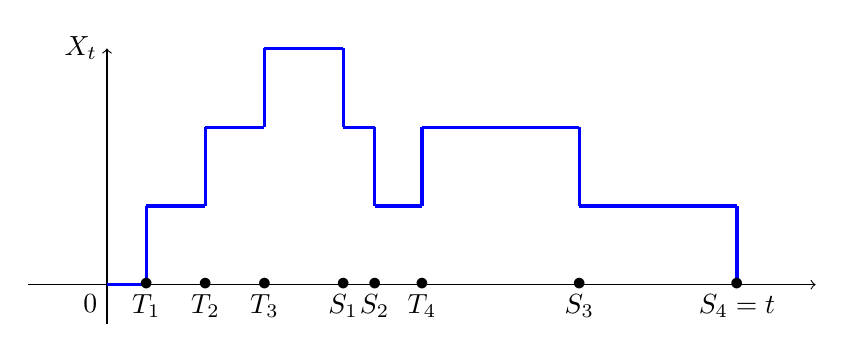
\begin{tikzpicture}
  %Origin and axis
  \coordinate (O) at (0,0);
  \draw[->] (-1,0) -- (9,0) coordinate[label = {below:$$}] (xmax);
  \draw[->] (0,-0.5) -- (0,3) coordinate[label = {left:$X_t$}] (ymax);
  %Lower linear boundary

 
  %Stochastic process trajectory
  
  \draw (0,0) node[blue,left] {} node{};
  \draw[very thick,blue,-] (0,0) -- (0.5,0) node[pos=0.5, above] {} ;
  \draw[very thick,blue] (0.5,0) -- (0.5,1) node[pos=0.5, right] {};
  \draw[very thick,blue,-] (0.5, 1) -- (1.25,1) node[pos=0.5, above] {};
  \draw[very thick,blue] (1.25,1) -- (1.25,2) node[pos=0.5, right] {};
  \draw[very thick,blue,-] (1.25,2) -- (2,2) node[pos=0.5, above] {};
  \draw[very thick,blue] (2,2) -- (2,3) node[pos=0.5, right] {};
  \draw[very thick,blue] (2,3) -- (3,3) node[pos=0.5, right] {};
  \draw[very thick,blue] (3,3) -- (3,2) node[pos=0.5, right] {};
  \draw[very thick,blue,-] (3,2) -- (3.4,2)node[pos=0.5, above] {};
  \draw[very thick,blue] (3.4,2) -- (3.4,1) node[pos=0.5, right] {};  
  \draw[very thick,blue,-] (3.4,1) -- (4,1) node[pos=0.5, above] {};
  \draw[very thick,blue] (4,1) -- (4,2) node[pos=0.5, right] {};  
  \draw[very thick,blue,-] (4,2) -- (6,2) node[pos=0.5, above] {};
  \draw[very thick,blue,-] (6,2) -- (6,1) node[pos=0.5, above] {};
   \draw[very thick,blue,-] (6,1) -- (8,1) node[pos=0.5, above] {};
    \draw[very thick,blue,-] (8,1) -- (8,0) node[pos=0.5, above] {};
     % \draw[very thick,blue,-] (,0.5) -- (8,0.5) node[pos=0.5, above] {};
     % \draw[very thick,blue,-] (8,0.5) -- (8,0) node[pos=0.5, above] {};
  %Jump Times
  \draw (0.5,0) node[black,below] {$T_1$} node{ \color{black}$\bullet$};
  \draw (1.25,0) node[black,below] {$T_2$} node{ \color{black}$\bullet$};
  \draw (2,0) node[black,below] {$T_3$} node{ \color{black}$\bullet$};
  \draw (3,0) node[black,below] {$S_1$} node{ \color{black}$\bullet$};
  \draw (3.4,0) node[black,below] {$S_2$} node{ \color{black}$\bullet$};
  \draw (4,0) node[black,below] {$T_4$} node{ \color{black}$\bullet$};
  \draw (6,0) node[black,below] {$S_3$} node{ \color{black}$\bullet$};
  \draw (8,0) node[black,below] {$S_4 =t$} node{ \color{black}$\bullet$};
  %Level of the counting process
   \draw (0,0) node[black,below left] {$0$} node{};
   % \draw (0,0.5) node[black,left] {$1$} node{ \color{black}$-$};
   % \draw (0,1) node[black,left] {$2$} node{ \color{black}$-$};
   % \draw (0,1.5) node[black,left] {$3$} node{ \color{black}$-$};
   % \draw (0,2) node[black,left] {$4$} node{ \color{black}$-$};
   % \draw (0,2.5) node[black,left] {$5$} node{ \color{black}$-$};

  % %Aggregated Capital gains
%  \draw (0,1.5) node[blue,below right] {$\mu_1$} node{ \color{blue}$-$};
%  \draw (0,2.25) node[blue,left] {$\mu_2$} node{ \color{blue}$-$};
%  \draw (0,3.75) node[blue,left] {$\mu_3$} node{ \color{blue}$-$};
  %Ruin time = First-crossing time time
%  \draw (5,0) node[black,above right] {${\tau_0}_u$} node{ \color{black}$\times$};
%  \draw[dotted,black] (0,3.28) -- (5,3.28);
%  \draw[dotted,black] (5,0) -- (5,3.28);
\end{tikzpicture}
\end{center}
\caption{Trajectoire du processus $X_t$ tel que $N_t = 4$.}
\label{fig:queue_little}
\end{figure}
La preuve consiste à calculer l'aire sous la courbe $A$ de deux façons. On a d'une part,
\begin{eqnarray*}
W &=& \frac{1}{N_t}\sum_{i=1}^{N_t}(S_i - T_i)\\
&=& \frac{(S_1 - T_1) + (S_2 - T_2) + (S_3-T_3) - (S_4-T_4)}{4}\\
&=&\frac{(S_4 - T_1) + (S_3 - T_4) + (S_2-T_2) + (S_1-T_3)}{4}\\
&=&\frac{A}{N_t}.
\end{eqnarray*}
On a d'autre part
\begin{eqnarray*}
L &=& \frac{1}{t}\int_0^t X_s\text{d}s\\
&=&\frac{1\cdot(T_2-T_1) + 2\cdot(T_3-T_2) + 3\cdot(T_3-S_1)+ 2\cdot(S_1-S_2) + 1\cdot(S_2 - T_4) + 2\cdot(T_4 - S_3) - 1\cdot(S_4 - S_3)}{t}\\
&=&\frac{A}{t}.
\end{eqnarray*}
On en déduit que 
$$
L = \frac{N_t}{t}W\rightarrow L = \lambda W.
$$
\end{proof}
Cette loi est très utile en pratique car on a parfois accès à $W$ facilement mais pas à $L$ ou inversement. On répond alors à des questions du type 
\begin{itemize}
	\item Quel est la longueur moyenne de la file d'attente?
	\item Si je vais au magasin, quel est mon temps d'attente moyen avant que le service commence?
	\item Quel est le temps moyen passé par un client dans le système?
\end{itemize}
\begin{ex}[file d'attente M/M/1 queue]
Supposons que le nombre de client arrivant dans le système est gouverné par un processus de Poisson d'intensité $\lambda$. Supposons ces unités sont servis par un unique serveur et que le temps de service soit une loi exponentielle de paramètre $\mu$. Le nombre de client dans le système est modélisé par un processus $X$. Ce processus est une file d'attente du type $M/M/1$ où $M$ signifie \textit{memoryless}. Le générateur du processus est donnée par 
$$
Q=\left(
\begin{array}{ccccccc}
-\lambda&\lambda&0&0&0&\cdots \\
\mu&-(\mu +\lambda)&\lambda&0&0&\cdots \\
0&\mu&-(\mu +\lambda)&\lambda&0&\cdots \\
0&0&\ddots&\ddots&\ddots &\vdots \\
\vdots&\vdots&\vdots&\vdots&\vdots&\vdots
\end{array}
\right).
$$
Il s'agit d'un processus de naissance mort dont les taux de naissance et de mort sont constants. La loi stationnaire existe si 
$$
S = \sum_{x = 1}^\infty\left(\frac{\lambda}{\mu}\right)^x <\infty,
$$
cela équivaut à $\lambda <\mu$ avec 
$$
S = \frac{\lambda}{\mu}\left(\frac{1}{1-\lambda / \mu}\right).
$$
On en déduit la loi stationaire du processus 
$$
\pi(x) = \left(1-\frac{\lambda}{\mu}\right)\left(\frac \lambda\mu\right)^x,\text{ pour }x\geq 0.
$$
Il s'agit d'une loi géométrique de paramètre $1-\lambda / \mu$. Le nombre moyen de clients dans le système est donc 
$$
L = \frac{\lambda}{\mu - \lambda}
$$
On en déduit le temps moyen passé dans le système via la loi de Little avec 
$$
W = \frac{L}{\lambda} = \frac{1}{\mu - \lambda}
$$
On peut considérer que la file d'attente comprend tous les client du système sauf celui en train d'être servi. Le temps moyen passé $W_q$ dans la file d'attente est donné par
$$
W_q = W - W_s, 
$$
où $W_s$ est le temps de service moyen. Il vient 
$$
W_q= \frac{\lambda}{\mu(\mu-\lambda)}.
$$
La longueur moyenne $L_q$ de la file d'attente peut être déterminé par la loi de Little en restreignant le système à la file d'attente. Il vient 
$$
L_q = \lambda W_q = \frac{\lambda^2}{\mu(\mu - \lambda)}.
$$


\end{ex}
De manière générale, un processus de type file d'attente atteint la stationarité lorsque les sorties du système dominent les entrées.
\section{Chaine de Markov subordonnée à un processus de Poisson}\label{sec:subordinated_poisson}
Soit $Y=(Y_n)_{n\geq 0}$ une chaine de Markov de matrice des transition $A$ sur un espace d'état $E$. On peut construire un processus de markov à partir de $Y$ et d'un processus de Poisson $N = (N_t)_{t\geq 0}$ d'intensité $\lambda$, indépendant de $Y$.
\begin{prop}\label{prop:subordinated_poisson}
Le processus défini par 
$$
X_t = Y_{N_t},\text{ }t\geq 0,
$$
est un processus de Markov de matrice des transitions données par 
$$
P_t = \exp[\lambda t(A - I)].
$$
\end{prop}
\begin{proof}
Soit $x,y \in E$
\begin{eqnarray*}
p_t(x,y) &=& \Prob(X_t = y|X_0 = x)\\
&=&\sum_{k=0}^\infty\Prob(X_t = y|X_0 = x, N_t = k)\Prob(N_t = k)\\
&=&\sum_{k=0}^\infty\Prob(Y_k = y|Y_0 = x)\frac{(\lambda t)^k\e^{-\lambda t} }{k!}\\
&=&\sum_{k=0}^\infty A^k_{x,y}\frac{(\lambda t)^k\e^{-\lambda t} }{k!}.
\end{eqnarray*}
On peut vérifier que c'est bien équivalent à \eqref{eq:transition_matrix_subordinated_poisson}. En effet, 
\begin{eqnarray*}
\exp[\lambda t(A - I)]&=& \sum_{k=0}^\infty\frac{(\lambda t^k}{k!}(A-I)^k\\
&=&\sum_{k=0}^\infty\frac{(\lambda t^k}{k!}\sum_{l=0}^k\binom{k}{l}A^l(-1)^{k-l}\\
&=&\sum_{k=0}^\infty\sum_{l=0}^k\frac{(\lambda t^k}{l!(k-l)!}A^l(-1)^{k-l}\\
&=&\sum_{l=0}^\infty\sum_{k=l}^\infty\frac{(\lambda t^k}{l!(k-l)!}A^l(-1)^{k-l}\\
&=&\sum_{l=0}^\infty \frac{A^l}{l!}\sum_{k=l}^\infty\frac{(\lambda t)^k}{(k-l)!}(-1)^{k-l}\\
&=&\sum_{l=0}^\infty A^l\frac{(\lambda t)^l}{l!}\e^{-\lambda t}\\
\end{eqnarray*}
Pour compléter la preuve on vérifie que pour $0= t_0<t_1<\ldots, t_n$ des instants et $x_0, x_1,\ldots, x_n$ des états de $E$, on a 
$$
\Prob(X_{t_0} = x_0, X_{t_1} = x_1,\ldots, X_{t_n}=x_n) = P_{t_1}(x_0,x_1)\ldots P_{t_n - t_{n-1}}(x_{n-1}, x_n).
$$
Il faut conditionner par rapport au valeur du processus $N$ aux temps $t_1,\ldots, t_n$ et c'est un peu fastidieux à écrire.
\end{proof} 
On peut identifier le générateur de $X$ par
$$
Q = \lambda(A-I).
$$
Inversement à partir d'un processus de Markov $X$ dont les temps de séjour sont bornées, $q_x <\lambda$ pour tout $x\in E$, on observe que 
$$
A = \frac{Q}{\lambda} + I
$$
est une matrice stochastique\footnote{Tous les coefficients sont positifs et les lignes se somment à $1$.}. Il ne faut toutefois pas confondre la chaine $Y$ de matrice des transition $A$ avec la chaine immergée Z définie plus haut!

\section{Loi \textit{phase-type}}\label{sec:phase_type}
Soit une processus de Markov $X=(X_t)_{t\geq 0}$ sur un espace d'état $E\cup\{\dagger\}$ comprenant un état absorbant caractérisés par un temps de séjour infini, soit
$$
q_\dag = 0.
$$
Le générateur de $X$ s'écrit alors par bloc avec 
$$
Q = \left(\begin{array}{c|c}
T&t\\
\hline
0&0
\end{array}\right),
$$
où $t$ et $T$ sont respectivement des vecteur et matrice carré de dimension $\text{Card}(E)$, tel que $t  + T \mathbf{1}_E = 0$, où $\mathbf{1}_E$ est un vecteur ne contenant que des $1$. Le vecteur $t$ correspond aux taux de transition vers l'état absorbant (les taux d'absorbtion) depuis chacun des état de $E$. Le temps d'absorbtion 
$$
\tau = \inf\{t\geq 0\text{ ; }X_t =\dagger\},
$$
suit une loi \textit{phase-type}, noté $\text{PH}(\alpha, T)$, où $\alpha$ est la loi initiale de $X$. Les lois $\textit{phase type}$ sont denses dans les lois de probabilité sur $\RL_+$\footnote{N'importe loi  sur $\RL_+$ peut s'écrire comme la limite d'une suite de loi \textit{phase type}.}. De nombreuses lois usuelles sont des cas particuliers de loi \textit{phase-type}.
\begin{ex}
\begin{enumerate}
	\item La loi $\ExpDist(\lambda)$ est une loi \textit{phase-type}, avec 
	$$
	\alpha = (\begin{array}{cc}1&0\end{array})\text{,  }Q = \left(\begin{array}{c|c}-\lambda & \lambda\\
	\hline
	0&0
	\end{array}\right).
	$$
    Schématiquement, 
\begin{center}
\begin{tikzpicture}[->, >=stealth', auto, semithick, node distance=3cm]
\tikzstyle{every state}=[fill=white,draw=black,thick,text=black,scale=0.8]
\node (0) {$$};
\node[state]    (1)[right of = 0]                     {$1$};
\node[state]    (2)[right of=1]   {$\dagger$};
\path
(0) edge[left, above]    node{$1$} (1)
(1) edge[left, above]    node{$\lambda$} (2)

% (2) edge[bend left]    node{$5/9$} (3)
% (3) edge[bend left]    node{$4/9$} (2)
% (3) edge[bend left]    node{$5/9$} (4)
% (4) edge[bend left]    node{$4/9$} (3)
% (4) edge[bend left]    node{$5/9$} (5)
% (5) edge[bend left]    node{$1$} (4)
;
\end{tikzpicture}
\end{center}
\item La loi $\GammaDist(k,\lambda)$, avec $k\in \mathbb{N}$, de densité 
$$
f(t) = \frac{\e^{\lambda t}\lambda^k t^{k-1}}{k!},\text{ pour }t>0,
$$
est une loi \textit{phase-type}, avec 
	$$
	\alpha = (\begin{array}{ccc}1& \cdots&0\end{array})\text{,  }
	Q = \left(
	\begin{array}{ccccc|c}
	-\lambda &\lambda&0&\cdots&0&0 \\
	0&-\lambda&\lambda&\cdots&0&0\\
	\vdots&0&\ddots&\ddots&\vdots&\vdots\\
	0&0&\cdots&0&-\lambda&\lambda\\
    \hline
    0&0&\cdots&0&0&0
	\end{array}
	\right).
	$$
    Schématiquement, 
\begin{center}
\begin{tikzpicture}[->, >=stealth', auto, semithick, node distance=3cm]
\tikzstyle{every state}=[fill=white,draw=black,thick,text=black,scale=0.8]
\node (0) {$$};
\node[state]    (1)[right of = 0]                     {$1$};
\node[state]    (2)[right of = 1]                     {$\cdots$};
\node[state]    (3)[right of = 2]                     {$k$};
\node[state]    (4)[right of=3]   {$\dagger$};
\path
(0) edge[left, above]    node{$1$} (1)
(1) edge[left, above]    node{$\lambda$} (2)
(2) edge[left, above]    node{$\lambda$} (3)
(3) edge[left, above]    node{$\lambda$} (4)

% (2) edge[bend left]    node{$5/9$} (3)
% (3) edge[bend left]    node{$4/9$} (2)
% (3) edge[bend left]    node{$5/9$} (4)
% (4) edge[bend left]    node{$4/9$} (3)
% (4) edge[bend left]    node{$5/9$} (5)
% (5) edge[bend left]    node{$1$} (4)
;
\end{tikzpicture}
\end{center}
\item La loi $\text{h-}\ExpDist(p,\lambda_1,\lambda_2)$, de densité 
$$
f(t) = p\lambda_1\e^{-\lambda_1 t} + (1 - p)\lambda_2\e^{-\lambda_2 t},\text{ pour }t>0.
$$
est une loi \textit{phase-type}, avec 
    $$
    \alpha = (\begin{array}{ccc}p& 1-p\end{array})\text{,  }
    Q = \left(
    \begin{array}{cc|c}
    -\lambda_1 &0&\lambda_1 \\
    0&-\lambda_2&\lambda_2\\
    \hline
    0&0&0
    \end{array}
    \right).
    $$
    Schématiquement, 
\begin{center}
\begin{tikzpicture}[->, >=stealth', auto, semithick, node distance=3cm]
\tikzstyle{every state}=[fill=white,draw=black,thick,text=black,scale=0.8]
\node (0) {$$};
\node (1)[right of = 0] {$$};
\node[state]   (2)[above of = 1] {$1$};
\node[state]    (3)[below of = 1] {$2$};
\node[state]    (4)[right of=1]   {$\dagger$};
\path
(0) edge[left, above]    node{$p$} (2)
(0) edge[left, below left]    node{$1-p$} (3)
(2) edge[left, above]    node{$\lambda_1$} (4)
(3) edge[left, below right]    node{$\lambda_2$} (4)

;
\end{tikzpicture}
\end{center}
\end{enumerate}
\end{ex}
Ces distributions donneNT une grande marche de manoeuvre à la modélisation. Leur représentation sous la forme de graph rend commode l'explication du modèle. On retrouve les lois \textit{phase type} dans de nombreux domaine d'application des probabilités. 
\begin{theo}
Soit $X$ une \va de loi $\text{PH}(\alpha, T)$, alors
\begin{enumerate}
    \item La fonction de répartition de $X$ est donnée par 
    $$
    F(x) = 1-\alpha\e^{Tx}\mathbf{1}_E
    $$
    \item La densité de $X$ est donnée par 
    $$
    f(x) = \alpha\e^{Tx}t
    $$
    \item L'espérance de $X$ est donnée par 
    $$
    \E(X) = -\alpha T^{-1}\mathbf{1}_E
    $$
    \item La fonction génératrice des moments $X$ est donnée par 
    $$
    M_X(\theta) = \E(\e^{\theta X}) = \alpha(-\theta I - T)^{-1}t
    $$
\end{enumerate}
\end{theo}
\begin{proof}
Voir \citet[Chapitre 9, Section 1]{Asmussen2010}
\end{proof}
En actuariat, les loi \textit{phase-type} sont utilisées pour
\begin{itemize}
    \item modéliser les montants de sinistres et le temps entre les sinistres, voir \citet{Bladt2005}, voir également la généralisation de \citet{Albrecher2019} pour permettre des distributions à queue lourdes
    \item modéliser la mortalité, voir \citet{Lin2007}
    \item modéliser l'entrée et le maintien en incapacité, voir \citet{Zadeh2013}
    \item valoriser des contrats de type épargne, voir\citet{Asmussen2019}
    \item tarifer via la théorie de la crédibilité, voir \citet{Zadeh2014}
\end{itemize}
L'estimation se fait par maximum de vraisemblance au moyen d'un algorithme d'espérance-maximisation (EM), voir \citet{Asmussen1996}. 
\begin{ex}
Le maintien en incapacité joue un rôle prépondérant en assurance emprunteur, et en prévoyance individuel. Les assurés ont généralement trois statuts
$$
\{\text{actif, incapable, décédé}\}
$$
qui peuvent former l'espace d'état $E$ d'un processus de Markov $X$ dont l'état absorbant est $\dagger = \text{décédé}$ et des aller-retours entre les états $\text{actif}$ et $\text{incapabale}$, comme sur la \cref{fig:transition_graph_disability}
\begin{figure}[!h]
 \begin{center}
\begin{tikzpicture}[->, >=stealth', auto, semithick, node distance=4cm]
% \tikzstyle{every state}=[fill=white,draw=black,thick,text=black,scale=0.8]
\tikzstyle{every state}=[rectangle,draw,rounded corners=4pt,fill=white]
\tikzstyle{test}=[diamond, aspect=2.5,thick, draw=blue,fill=yellow!50,text=blue] 

\node[test]    (1)               {$\text{Valide}$};
\node[test]    (2)[right of=1]   {$\text{Incapacité}$};
\node[state]    (3)[below right of=1]   {$\text{Décès}$};

\path
(1) edge[bend left] node[above]{} (2)
(2) edge[bend right] node[above]{} (1)
(1) edge[left]  node{} (3)
(2) edge[left]  node{} (3)
;
\end{tikzpicture}
\end{center}
\caption{Les états des assurés dans le cadre de la modélisation du maintien en incapacité}
\label{fig:transition_graph_disability}
\end{figure}
Le modèle  se complexifie en distinguant les différentes classes d'age $j=1\ldots, l$ associées à des taux d'entrée en incapacité distincts
$$
\beta_1,\ldots, \beta_l,
$$
des taux de retour à l'activité distincts
$$
\gamma_1,\ldots, \gamma_l,
$$
des taux de transitions de classes 
$$
\zeta_1,\ldots, \zeta_{l-1},
$$
et finalement des taux de décès distincts
$$
\delta_1,\ldots, \delta_l.
$$
Le modèle complet est donnée par le graph suivant:
\begin{figure}[ht!]
\begin{center}
\begin{tikzpicture}[->, >=stealth', auto, semithick, node distance=2cm]
\tikzstyle{every state}=[fill=white,draw=black,thick,text=black,scale=0.8]
\node[state]   (1) {Valide $1$};
\node[state]   (2)[right of = 1] {$\ldots$};
\node[state]   (3)[right of = 2] {Valide $l$};
\node[state]   (4)[below of = 1] {Incap $1$};
\node[state]   (5)[below of = 2] {$\ldots$};
\node[state]   (6)[below of = 3] {Incap $l$};
\node (7)[above of = 1] {};
\node (8)[above of = 3] {};
\node (9)[below of = 4] {};
\node (10)[below of = 6] {};

\path
(1) edge[bend left, above]    node{$\zeta_1$} (2)
(2) edge[bend left, above]    node{$\zeta_{l-1}$} (3)
(4) edge[bend right, below]    node{$\zeta_1$} (5)
(5) edge[bend right, below]    node{$\zeta_{l-1}$} (6)
(1) edge[bend right, left]    node{$\beta_1$} (4)
(3) edge[bend right, left]    node{$\beta_{l}$} (6)
(4) edge[bend right, right]    node{$\gamma_1$} (1)
(6) edge[bend right, right]    node{$\gamma_{l}$} (3)
(1) edge[right, left]    node{$\delta_1$} (7)
(3) edge[right, left]    node{$\delta_l$} (8)
(4) edge[right, left]    node{$\delta_1$} (9)
(6) edge[right, left]    node{$\delta_l$} (10)

% (4) edge[bend right, below]    node{$\zeta_1$} (5)
% (5) edge[bend right, below]    node{$\zeta_{l-1}$} (6)
% (2) edge[left, above]    node{$\lambda_1$} (4)
% (3) edge[left, below right]    node{$\lambda_2$} (4)
;
\end{tikzpicture}
\end{center}
\label{fig:transition_graph_ph}
\end{figure}
Il ne reste plus qu'à construire la matrice $T$ :).

\end{ex}


\begin{thebibliography}{11}
\providecommand{\natexlab}[1]{#1}
\providecommand{\url}[1]{\texttt{#1}}
\expandafter\ifx\csname urlstyle\endcsname\relax
  \providecommand{\doi}[1]{doi: #1}\else
  \providecommand{\doi}{doi: \begingroup \urlstyle{rm}\Url}\fi

\bibitem[Albrecher and Bladt(2019)]{Albrecher2019}
Hansjörg Albrecher and Mogens Bladt.
\newblock Inhomogeneous phase-type distributions and heavy tails.
\newblock \emph{Journal of Applied Probability}, 56\penalty0 (4):\penalty0
  1044--1064, dec 2019.
\newblock \doi{10.1017/jpr.2019.60}.

\bibitem[Asmussen and Albrecher(2010)]{Asmussen2010}
S{\o}ren Asmussen and Hansjörg Albrecher.
\newblock \emph{Ruin Probabilities}.
\newblock {WORLD} {SCIENTIFIC}, sep 2010.
\newblock \doi{10.1142/7431}.

\bibitem[Asmussen et~al.(2019)Asmussen, Laub, and Yang]{Asmussen2019}
S{\o}ren Asmussen, Patrick Laub, and Hailiang Yang.
\newblock Phase-type models in life insurance:fitting and valuation of
  equity-linked benefits.
\newblock \emph{Risks}, 7\penalty0 (1):\penalty0 17, feb 2019.
\newblock \doi{10.3390/risks7010017}.

\bibitem[Asmussen et~al.(1996)Asmussen, Nerman, and Olsson]{Asmussen1996}
Søren Asmussen, Olle Nerman, and Marita Olsson.
\newblock Fitting phase-type distributions via the em algorithm.
\newblock \emph{Scandinavian Journal of Statistics}, 23\penalty0 (4):\penalty0
  419--441, 1996.
\newblock ISSN 03036898, 14679469.
\newblock URL \url{http://www.jstor.org/stable/4616418}.

\bibitem[Bladt(2005)]{Bladt2005}
Mogens Bladt.
\newblock A review on phase-type distributions and their use in risk theory.
\newblock \emph{{ASTIN} Bulletin}, 35\penalty0 (1):\penalty0 145--161, may
  2005.
\newblock \doi{10.1017/s0515036100014100}.

\bibitem[Dobrow(2016)]{Dobrow2016}
Robert~P. Dobrow.
\newblock \emph{Introduction to Stochastic Processes With R}.
\newblock John Wiley {\&} Sons, Inc, mar 2016.
\newblock \doi{10.1002/9781118740712}.

\bibitem[Lin and Liu(2007)]{Lin2007}
X.~Sheldon Lin and Xiaoming Liu.
\newblock Markov aging process and phase-type law of mortality.
\newblock \emph{North American Actuarial Journal}, 11\penalty0 (4):\penalty0
  92--109, oct 2007.
\newblock \doi{10.1080/10920277.2007.10597486}.

\bibitem[Little(1961)]{Little1961}
John D.~C. Little.
\newblock A proof for the queuing formula:{L}= $ \lambda${W}.
\newblock \emph{Operations Research}, 9\penalty0 (3):\penalty0 383--387, jun
  1961.
\newblock \doi{10.1287/opre.9.3.383}.

\bibitem[Truquet(2015)]{Truquet_stat_proc}
Lionel Truquet.
\newblock Statistiques des processus 3a.
\newblock Lecture notes, 2015.
\newblock
  \url{https://ensai.fr/wp-content/uploads/2019/06/polystatdesprocessus2.pdf}.

\bibitem[Zadeh and Stanford(2014)]{Zadeh2014}
Amin~Hassan Zadeh and David~A. Stanford.
\newblock Bayesian and bühlmann credibility for phase-type distributions with
  a univariate risk parameter.
\newblock \emph{Scandinavian Actuarial Journal}, 2016\penalty0 (4):\penalty0
  338--355, jun 2014.
\newblock \doi{10.1080/03461238.2014.926977}.

\bibitem[Zadeh et~al.(2013)Zadeh, Jones, and Stanford]{Zadeh2013}
Amin~Hassan Zadeh, Bruce~L. Jones, and David~A. Stanford.
\newblock The use of phase-type models for disability insurance calculations.
\newblock \emph{Scandinavian Actuarial Journal}, 2014\penalty0 (8):\penalty0
  714--728, mar 2013.
\newblock \doi{10.1080/03461238.2012.761645}.

\end{thebibliography}

\newpage